\documentclass[xodstep]{wnspt}

\author   {Tetiana Mossur}
\nralbumu {76716}
\kierunek {Informatyka}
\specjalnosc {Programowanie}
\date     {2024}
\miejsce {Cz\k{e}stochowa}
%\instytut {Zak\l{}adzie Informatyki Stosowanej}
\opiekun  {dr hab. Andrzeja Zbrzeznego}

\usepackage{amsmath}
\usepackage{amsfonts}
\usepackage{amsthm}
\usepackage{amssymb}
\usepackage[T1]{fontenc}
\usepackage[utf8]{inputenc}
\usepackage[polish]{babel}
\usepackage{polski}
\usepackage{csquotes}
\usepackage{times}
\usepackage{colortbl}
\usepackage{graphicx}
\usepackage{url}
\usepackage{setspace}
\usepackage{indentfirst}
\usepackage{listingsutf8}
\usepackage{beramono}
\usepackage[%
backend=biber,refsegment=section,
defernumbers=true,
]{biblatex}

\usepackage{fontspec}
\setmainfont{Carlito}

\bibliography{literatura}

\lstset{ %
language=Python,                  % choose the language of the code
basicstyle=\ttfamily,           % the fonts that are used for the code
numbers=left,                   % where to put the line-numbers
numberstyle=\footnotesize,      % the size of the fonts that are used for the line-numbers
stepnumber=1,                   % the step between two line-numbers. If it's 1 each line will be
numbersep=5pt,                  % how far the line-numbers are from the code
showspaces=false,               % show spaces adding particular underscores
showstringspaces=false,         % underline spaces within strings
showtabs=false,                 % show tabs within strings adding particular underscores
frame=single,                   % adds a frame around the code
tabsize=4,                      % sets default tabsize to 2 spaces
captionpos=b,                   % sets the caption-position to bottom
breaklines=true,                % sets automatic line breaking
breakatwhitespace=false,        % sets if automatic breaks should only happen at whitespace
escapeinside={\%*}{*)}          % if you want to add a comment within your code
}

\newcommand{\R}{mathbb{R}}

\renewcommand{\lstlistlistingname}{Spis listingów}
\renewcommand{\lstlistingname}{Listing}

\newtheorem{lemat}{Lemat}
\newtheorem{twierdzenie}{Twierdzenie}

\title{Efektywność SMT solverów dla klasycznych problemów NP-trudnych
\\{~}
\\{~}
Effectiveness of SMT solvers for classical NP-hard problems}

\frenchspacing

\begin{document}
\begin{abstract}
Celem niniejszej pracy jest analiza i ocena efektywności SMT solverów w rozwiązywaniu klasycznych problemów zaliczanych do klasy NP-trudnych. Przełom w informatyce teoretycznej sprawił, że tego rodzaju zagadnienia stały się przedmiotem intensywnych badań. Niniejsza praca skupi się na zrozumieniu, jak Satisfiability Modulo Theories (SMT) solvery, będące potężnym narzędziem w dziedzinie rozstrzygania logicznego, radzą sobie z tymi wyjątkowo wymagającymi problemami.
Przedmiotem badań będą klasyczne problemy NP-trudne, a celem jest zbadanie i porównanie efektywności SMT solverów Pythona - Z3, Yices i CVC5 - w kontekście rozwiązywania konkretnych problemów. Wybór tych narzędzi wynika z ich popularności, wszechstronności i aktywnego udziału w społeczności badawczej.

\end{abstract}

\keywords{SMT, SMT-solvery, Z3, Yices, CVC5, Python, złożoność obliczeniowa, NP-hard}
\maketitle
\onehalfspacing
%\setlength{\footskip}{20pt}

\introduction

Celem niniejszej pracy jest zbadanie skuteczności SMT solverów Pythona, a mianowicie Z3, Yices oraz CVC5 w rozwiązywaniu problemów NP-trudnych, takich jak: ... .

W pierwszym rozdziale zawarłam teoretyczne fundamenty problemów NP-trudnych oraz wprowadziłam kontekst, w którym operują SMT solvery. Zdefiniowałam charakterystykę tych problemów i omówiłam kluczowe koncepcje teoretyczne.

Rozdział drugi przedstawia obszerny przegląd literatury z zakresu SMT solverów oraz problemów NP-trudnych. Poprzez analizę wcześniejszych badań, podkreśliłam istotne osiągnięcia oraz ewentualne luki w dotychczasowym rozumieniu tej dziedziny, co stanowi podstawę dla dalszej analizy i eksperymentów.

W rozdziale trzecim zawarłam szczegółowy opis wybranych problemów obliczeniowych oraz SMT solverów, skupiłam się na praktycznych aspektach funkcjonowania tych narzędzi, ich mocnych stronach i potencjalnych ograniczeniach.

Rozdział czwarty poświęcony jest praktycznym eksperymentom, wykorzystując Z3, Yices i CVC5 do rozwiązania wybranych problemów NP-trudnych. Analiza wyników pozwoli określić efektywność poszczególnych solverów i wyciągnąc wnioski co do ich zastosowania.

\chapter{Teoretyczne podstawy SMT i klasy NP-hard}
\section{Wymagania biznesowe}
\section{Słownik skrótów i pojęć}
\cite{java_fundamentals}
\section{Wymagania funkcjonalne użytkowników}
%\subsection*{Hierarchia grup użytkowników przedstawiona graficznie}
\subsection{Wymagania funkcjonalne użytkownika niezarejestrowanego}
\subsection{Wymagania funkcjonalne użytkownika zarejestrowanego}
\subsection{Wymagania funkcjonalne administratora}
\subsection{Wymagania funkcjonalne dziennikarz}
\subsection{Wymagania funkcjonalne marketing}
\subsection{Wymagania funkcjonalne specjalista danych}
\subsection{Wymagania funkcjonalne super administratora}
\section{Wymagania niefunkcjonalne użytkowników}
\section{Wymagania niefunkcjonalne systemowe}
\section{Reguły biznesowe}
\cite{java17doc}


\chapter{Problemy NP-trudne}

Załóżmy, że jesteśmy menedżerem logistyki, który musi zoptymalizować harmonogram dostaw towarów przez park pojazdów w warunkach ograniczonej sieci dystrybucyjnej obejmującej całe miasto. To pozornie rutynowe zadanie, po bliższym przyjrzeniu się, okazuje się być złożonym problemem optymalizacji kombinatorycznej, charakteryzującym się potrzebą minimalizacji kosztów paliwa, skrócenia czasu podróży i maksymalizacji przepustowości dostaw.

W poszukiwaniu optymalnego rozwiązania mamy do czynienia ze stale rosnącym zestawem zmiennych, w tym nieprzewidywalną dynamiką ruchu, różnymi rozmiarami paczek i dynamicznymi zmianami popytu ze strony klientów. Każda decyzja o ustaleniu konkretnych tras dostawy lub nadaniu priorytetu określonym miejscom docelowym powoduje eksplozję kombinatorycznych możliwości, zmieniając problem optymalizacji logistycznej w przykład problemu NP-trudnego.

Z perspektywy obliczeniowej, problemy NP-trudne są klasą problemów, dla których nie istnieje algorytm wielomianowy, który może zapewnić optymalne rozwiązanie we wszystkich przypadkach. Złożoność ta jest wyraźnie widoczna w problemach takich jak optymalizacja tras, gdzie ogromna przestrzeń rozwiązań nie pozwala na proste rozwiązanie. Złożoność takich problemów logistycznych odzwierciedla szersze trudności występujące w problemach NP-trudnych w różnych obszarach obliczeniowych i optymalizacyjnych.

\section{Złożoność obliczeniowa}

\section{Problem spełnialnośći}

\section{Definicja klasy problemów NP-trudnych}



%\begin{lstlisting}
%\end{lstlisting}
 

\chapter{Opis wykorzystywanych narzędzi}
%Rozdział opisuje zastosowanie 

\section{Z3 Solver}
Z3 to wydajny SMT solver dostępny bezpłatnie przez Microsoft Research. Z3 jest solverem dla logiki symbolicznej, będącej podstawą wielu narzędzi inżynierii oprogramowania. Solwery SMT polegają na ścisłej integracji wyspecjalizowanych silników walidacyjnych. Każdy silnik jest elementem ogólnej struktury i implementuje wyspecjalizowane algorytmy. Przykładowo, silnik Z3 dla arytmetyki obejmuje Simplex, cięcia i rozumowanie wielomianowe, podczas gdy silnik dla obsługi ciągów znaków i wyrażeń regularnych korzysta z metod symbolicznych pochodnych języków regularnych. Wspólną cechą wielu algorytmów jest sposób, w jaki wykorzystują dwoistość między znajdowaniem rozwiązań spełniających a dowodów odrzucających. Solver ten integruje również silniki do wnioskowań globalnych i lokalnych oraz globalnej propagacji.
Z3 jest używany w szerokim zakresie zastosowań inżynierii oprogramowania, obejmując weryfikację programów, walidację kompilatorów, testowanie, fuzzing przy użyciu dynamicznego wykonywania symbolicznego, rozwój oprogramowania oparty na modelach, weryfikację sieci i optymalizację.
Z3 może być zbudowany przy użyciu Visual Studio, pliku Makefile lib CMake. Zapewnia obsługę wielu języków programowania, w tym .NET, C, C++, Java, OCaml, Web Assembly i Python.

\subsection{Architektura systemu}
	\begin{figure}
	\centering
	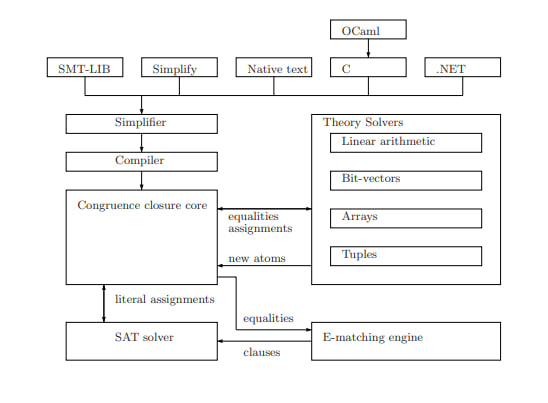
\includegraphics[width=0.7\linewidth]{screenshot001}
	\caption{}
	\label{fig:screenshot001}
	\end{figure}
\text{Z3 integruje nowoczesny solver SAT oparty na DPLL, bazowy solwer dla teorii, który obsługuje równości i funkcje nieinterpretowane, specjalistyczne silniki (dla arytmetyki, tablic itp.) oraz maszynę abstrakcyjną E-matching (dla kwantyfikatorów). Z3 jest zaimplementowany w C++. Schematyczny przegląd Z3 pokazano na poniższym rysunku.}

\textbf{Simplifier}. Formuły wejściowe są najpierw przetwarzane przy użyciu niekompletnego, ale wydajnego uproszczenia. Simplifier stosuje standardowe zasady redukcji algebraicznej, takie jak $p \land true \implies p$, ale także wykonuje ograniczone uproszczenie kontekstowe, identyfikując definicje równościowe w danym kontekście i redukuje pozostałą formułę przy użyciu definicji, na przykład $x = 4 \land q(x) \implies x = 4 \land q(4)$. Trywialnie spełnialny spójnik $x = 4$ nie jest kompilowany do jądra, ale zachowany poza nim na wypadek, gdyby klient wymagał modelu do obliczenia x.

\textbf{Compiler}. Uproszczona abstrakcyjna reprezentacja drzewa składniowego formuły jest przekształcana w inną strukturę danych, składającą się z zestawu klauzul i węzłów domknięcia kongruencji.


\section{Yices Solver}
sdcssdsdf

\section{CVC5 Solver}
sdsdcfsdfcdsf
\chapter{Kodowanie problemów}


\summary
Celem mojej pracy było zapoznanie czytelnika z ... 
Uważam, że udało mi się zrealizować ten cel. Starałem się opisać zarówno ...

% załączniki (opcjonalnie):
\appendix
\chapter{Tytuł załącznika jeden}
Treść załącznika jeden.

\chapter{Tytuł załącznika dwa}
Treść załącznika dwa.

%\bibliographystyle{plain}
%\bibliography{literatura}

\printbibliography[type=article, title={Bibliografia - artykuły}]
\printbibliography[type=book,title={Bibliografia - książki}]
\printbibliography[type=misc,title={Bibliografia - strony internetowe}]

% spis tabel (jeżeli jest potrzebny):
\listoftables

% spis rysunków (jeżeli jest potrzebny):
\listoffigures

% spis listingów (jeżeli jest potrzebny):
\lstlistoflistings

\end{document}
